%Throughout this review, we will consider the relic density as a rough order-of-magnitude guide for our selection of models and results, rather than as an exact constraint. Most of the models considered that satisfy the relic density only consider a single particle. The DM sector may be much more complex than a single particle with a limited number of interaactions. Nevertheless, if these simple examples dominate over others.  

%these simple examples may emerge in the searches at the early stages of the LHC  particles  

In this chapter, we will link the observations on DM to its particle properties. We then enumerate the possible reactions of DM at the LHC within certain grounding assumptions, building from simple to more complex models in terms of particle content. 

\subsection{Observations on DM as a guide for its particle properties}
\label{sec:DMObservations}

The observations mentioned in Section~\ref{sec:intro} require the dark matter particle to be stable on a cosmological timescale. This has important consequences for the prediction and observation of dark matter reactions at colliders. 

Firstly, a simple theoretical way to stabilize DM is the introduction
of a global $Z_2$ symmetry, as in Ref.~\cite{Batell:2010bp}. A realization of this
symmetry can be found in R-parity in the MSSM. %citation?
Under this symmetry, the parity of the DM particle is odd, while the parity of SM particles is even. 
$Z_2$-parity is multiplicative and conserved: this 
%is Z_2 parity a thing? I don't want to have it confused with the global SM parity
implies that an odd-parity DM particle (charge -1) cannot decay into any 
lighter even-parity SM particles (charge +1) and it is therefore stable. 
Additionally, DM particles will be produced in pairs from the decay of other particles
that are charged under the same gauge group as the SM. 

A simplified diagram of an s-channel process at colliders satisfying $Z_2$ symmetry is shown in panel (b) of Fig.~\ref{fig:monoX}.
If the particle mediating the SM-DM interaction is a SM particle, no additional particles beyond the DM need to be invoked, leading to the simplest DM production mode at the LHC. The only theoretically viable SM portal particles within the grounding assumptions of this revew are the Z and the Higgs bosons, described in Section~\ref{sec:HZPortalModels}. 

%TODO: add sidebar figure of s-channel. 
%this will become useful when we talk about s-channel mediators. maybe also make a point
%for the t-channel mediator?

Secondly, dark matter particles are invisible to detectors. 
However, the rest of the event is not: one can observe DM particles
produced in the event and escaping the detector 
due to their missing momentum in the transverse plane, 
if they recoil against one or more visible SM particles. 

\begin{marginnote}[]
Transverse momentum is denoted as \pt in this review, 
and the magnitude of the missing transverse momentum is 
termed \MET. 
\end{marginnote}
%CD: CMS uses this in all its plots, but i don't find it too relevant yet
%From: https://arxiv.org/pdf/1106.5048.pdf
%The following notation is used: the vector boson momentum in the transverse plane is ?qT, and the hadronic recoil, defined as the vector sum of the transverse momenta of all particles except the vector boson (or its decay products, in the case of Z candidates), is ?uT. Momentum conservation in the transverse plane requires ?qT + ?uT = 0. The recoil is the negative of the induced ?E/T.

%I don't like how this is linking up. 

%shared context: many possible new physics searches at the LHC
%problem: can't do them all
%solution: strong theoretical motivation, as well as observability
%exposition: particular case of DM

Collider experiments have a nearly unlimited choice of theoretically
motivated DM targets to search for. 
Theoretical arguments alone are not sufficient for a DM model to be tested at the LHC: 
couplings to SM particles need to feature in the model and be sufficiently large
to produce new particles and observe their signatures in the detectors. 

%everyone thinks of WIMPs, how strong is strong, how weak is weak? quantitative question of coupling, depends on model. in the introduction: need to talk about DM properties. Weak enough that there is no visible EM signal (no light emission or absorption). Relate those properties to what the particle physics properties need to be. Have a model in mind: s-channel mediator between DM and SM, weakness of interaction comes from particle being heavy or coupling being small. DMF models have order=1 couplings. 

Models of particle dark matter include SM couplings to satisfy cosmological observations in the freeze-out case. These couplings need to be weak enough that there is no visible signal of DM particles, as there is no evidence for DM interacting strongly with baryonic matter, nor for its emission or absorption of light. A typical DM-SM coupling satisfying relic density is of the order of XXX. %CD: isn't this too model-dependent?

The only SM particle that satisfies the requirement of being sufficiently weakly interacting is the neutrino. However, neutrinos cannot make up the totality of DM as they 
%are not sufficiently massive 
are relativistic particles and cannot explain the galaxy structures that formed in the universe~\cite{PlehnLecturesDM}. %%CITE FENG AR, BERTONE'S BOOK
%The upper bound on the neutrino content of DM is YYY. Not sure where to find this number

Unlike previous accelerators that either yielded large datasets (e.g. B-factories) or high center-of-mass energy (e.g. Tevatron), the LHC gives unprecedented access to both rare processes and high scale processes at the same time, planning to collect 3/ab by 2035 reaching the design center-of-mass energy of 14 TeV. For this reason, it is worth speculating whether the portal particles could be observed at the LHC for the first time. Models that include one or more very massive new particles beyond the SM in addition to the DM particle are also an LHC search target, and are described in Section~\ref{sec:BSMMediatorModels}. 

Portal models and models of simple BSM mediation are only motivated by the observation of DM. They keep the SM and the DM sectors separate, and make no claim to being a solution of other shortfalls of the SM. However, the coincidence that hierarchy problem, gauge coupling unification and DM particle nature could be solved with a single theory with observable consequences at the electroweak scale, has been one of the driving reasons to develop and consider SuperSymmetry (SUSY) as one of the main search targets for LHC searches. These models are discussed in Section~\ref{sec:SUSYModels}.

Finally, let us return on the concept of observability of the search target mentioned above. Even general purpose particle detectors may miss certain classes of phenomena, as the initial design choices privileged searches for the Higgs boson and for particles that generally decay promptly, as predicted by models discussed so far. However, there is tension when confronting data with portal models, BSM mediation models and supersymmetric models that are compatible with the standard freeze-out scenarios. This encourages us to look for other classes of models, especially those including particles with long lifetimes, as a way to shine the search lamppost beyond the classic WIMP scenario. Reaction including those particles and their connections to DM are sketched in Section~\ref{sec:LLPModels}

\subsection{Caveats and grounding assumptions}
\label{sec:GroundingAssumptions}

%%I suggest this part goes in the introduction, as it motivates enumeration of models in chapter 2 and comparisons in chapter 4. 
The observation of a signal of visible or invisible particles at an LHC experiment that could be identified as being generated by one of the reactions described in this chapter cannot lead to claim that DM has been discovered. This is because DM is stable on a cosmological scale, while LHC experiments are limited to the observation of particles with a lifetime that is longer than the time needed to escape the detector (i.e. DM candidate particles could still decay into other particles outside the detector and leave a signal of missing transverse momentum). This is not a reason to discount searches for DM at the LHC, as such a signal would still be a groundbreaking discovery, regardless of its interpretation. This statement highlights the importance of the comparison of LHC results, where DM would be produced in the lab, with the results of complementary experiments that look for signals of DM coming from space. This comparison can only take place if the same theoretical model is used to interpret both results. This motivates the enumeration of possible models in this chapter. 

To define the scope of the reactions for invisible particles at colliders considered in this review, we make a number of grounding assumptions: 

\begin{enumerate}

\item We describe models where the DM particle interacts with SM particles, either directly or indirectly;
\item We restrict our list to models that include a $Z_2$ symmetry to stabilize DM;
\item We privilege models that respect Minimal Flavour Violation (MFV), which imposes that the flavor structure of couplings between DM and ordinary particles follows that of the SM.  %CITE?
%Citation from DMFs
%[49] J. Abdallah, H. Araujo, A. Arbey, A. Ashkenazi, A. Belyaev, et al., Simplified models for dark matter searches at the LHCSubmitted to Phys.Dark Univ. arXiv:1506.03116.
% [47] A. A. Petrov, W. Shepherd, Searching for dark matter at LHC with mono- Higgs production, Phys.Lett. B730 (2014) 178–183. arXiv:1311.1511, doi:10.1016/j.physletb.2014.01.051.
% [51] R. S. Chivukula, H. Georgi, Composite Technicolor Standard Model, Phys.Lett. B188 (1987) 99. doi:10.1016/0370-2693(87)90713-1.
% [52] L. Hall, L. Randall, Weak scale effective supersymmetry, Phys.Rev.Lett. 65 (1990) 2939–2942. doi:10.1103/PhysRevLett.65.2939.
% 2570 [53]
% A. Buras, P. Gambino, M. Gorbahn, S. Jager, L. Silvestrini, Universal unitarity triangle and physics beyond the Standard Model, Phys.Lett. B500 (2001) 161–167. arXiv:hep-ph/0007085, doi:10.1016/S0370-2693(01) 00061-2.
% 2575
% [54] G. D’Ambrosio, G. Giudice, G. Isidori, A. Strumia, Minimal Flavor Viola- tion: An effective field theory approach, Nucl.Phys. B645 (2002) 155–187. arXiv:hep-ph/0207036, doi:10.1016/S0550-3213(02)00836-2.
\item We primarily consider models where DM is a Dirac fermion, relying on existing theory material developed for early Run-2 searches. Other cases yield similar phenomenology for LHC searches, with some exceptions that we describe in this chapter. 
\item We privilege models that have a connection with thermal relic from freeze-out. We remark however that there are other models from other cosmological histories (e.g. freeze-in) that can be considered and would lead to interesting LHC signatures~\cite{Bernal:2017kxu}. 
%The Dawn of FIMP Dark Matter: A Review of Models and Constraints  - https://arxiv.org/pdf/1706.07442.pdf, Minimal Decaying Dark Matter and the LHC - https://arxiv.org/pdf/1305.6587.pdf
%
\end{enumerate}

%Caveat??
In the following sections will describe models from the perspective of experimental collider physicists, focusing on a selection of models that provide distinct and testable LHC signatures, without the ambition of theoretical completeness. For other perspectives on the models used for early LHC searches for DM, see~\cite{Kahlhoefer:2017dnp,Abercrombie:2015wmb,Arcadi:2017kky,Ellis:2010kf}. %Cite SUSY review by Feng?

\subsection{Higgs and Z boson portals}
\label{sec:HZPortalModels}

Even if we cannot observe DM itself at colliders, we can look for visible particles that are associated to Dark Matter. The LHC alone cannot solve the strong CP problem through observation of the axion, but it can still observe e.g. scalar resonances that appear in the theory. %CD: I think axion is out of place here

This raises the question of whether any of the SM particles could be associated to DM, for example in a similar fashion as the W and Z bosons mediate the weak interaction and produce neutrino pairs in the reaction. Models where the SM particle sector is coupled to the dark sector through an existing or a new particle are called \textit{portal models}. This kind of model leads to the most economical particle content for reactions at the LHC, as one only needs to add a neutral DM particle to the SM content if one of the SM particles is the portal particle. SM fermions cannot be portal particles under the assumption of a $Z_2$ symmetry, as they would allow the decay of DM. Photons, W bosons and gluons can't be portal particles either, as DM does not absorb nor emit light, nor it does it have electromagnetic or strong charge. The only viable SM portal particles remaining are the Z and the Higgs bosons. 

There are strong theoretical and experimental arguments to explore SM portal models at the LHC. 
%Theoretical
Processes involving mediators at the electroweak scale are among the first to be investigated, in DM theories that predict new weakly interacting particles~\cite{Cotta:2012nj}. This kind of portals are also present in a number of other theories~\cite{Arcadi:2014lta}. %CD: are there earlier monoZ papers?
%Experimental 
However, it is only the recent generations of collider and direct detection experiments that have started being able to probe the range of small couplings and relatively large scales required to observe this kind of models. 

\subsubsection{Z portal models}

The \textbf{Z portal} model, where the DM particle has vector and axial vector interactions with a Z boson, is a minimal extension of the SM as it only requires a single new particle to be added to the SM particle content. In $SU(2)_L \times U(1)$ extensions of the SM, the axial and vector couplings of the Z boson to DM are generally required to be of the same order. If no other couplings are present, this model is not $SU(2) \times U(1)$ invariant, unless couplings to the DM to the Higgs boson are added as well~\cite{Kahlhoefer:2015bea}. 
%The couplings between the Z and the DM can be vector, axial or mixed. 
In the minimal case where the couplings do not depend on the Lorentz structure of the interaction, 
%what I want to say: In general they are excluded in their minimal version because of their strong vectorial coupling necessary to respect relic abundance bounds.
large couplings are required for this model to satisfy the relic density. 
In the case of equal vector and axial couplings, this model is heavily constrained by LEP and direct detection experiments (see e.g. Refs.~\cite{Arcadi:2014lta,Escudero:2016gzx}). This model can still be viable wherever no relations between the vector and axial couplings are present. A review of Z portal models with different couplings can be found in Ref.~\cite{Arcadi:2014lta}. 
%Does one require a certain kind of couplings for symmetries? 
%Arcadi says: 
%In all these extensions, the axial coupling Aχ (see eq.(1)) of the Z boson to the dark matter is naturally of the order of magnitude of its vectorial coupling Vχ. The deep reason is that in a framework of SU(2)L × U(1) breaking the original SU(2)L condition (Vχ = Aχ) is only mildly modified by the dynamic of the breaking. 
%Maybe link this to the choices for the Z' model later on? 

\subsubsection{Higgs portal models}

The discovery of a SM-like Higgs boson~\cite{Aad:2012tfa,Chatrchyan:2012xdj} has sparked theoretical and experimental interest in \textbf{Higgs portal} models, where DM particles can interact with SM particles only through the Higgs boson (see e.g. Refs.~\cite{Patt:2006fw,Englert:2011yb,Djouadi:2011aa}). In Higgs portal models, DM couples to the SM operator connecting two Higgs fields and could dominate the interactions between SM and DM sectors.
%since the $H\dagger H$ operator has the lowest dimension in the SM. 
This interaction is renormalizable and leads to a UV-complete, minimal theory in the case of scalar and vector DM, while a self-consistent theory requires the presence of further particles mediating the interaction in the case of fermion DM~\cite{Freitas:2015hsa,Escudero:2016gzx,deSimone:2014pda}. %and references therein? In case there is more room for H portal citations, should cite also: 
%https://arxiv.org/pdf/1304.2417.pdf
%From Escudero:2016gzx
%We point out that for fermionic dark matter heavier than several TeV, perturbative unitarity is lost, and higher dimension operators such as those ones considered in ref. [10] may become relevant for the phenomenology. It is interesting to note that within the context of the MSSM, a bino-like neutralino (with a subdominant higgsino fraction) can possess the characteristics found within this scenario [11].


%The couplings of the Higgs to DM can be scalar or pseudoscalar. This may need to be discussed later. 

%Another completion of the Dirac DM:
%S. Baek, P. Ko, and W.-I. Park, Search for the Higgs portal to a singlet fermionic dark matter at the LHC, J. High Energy Phys. 1202 047, (2012), [arXiv:1112.1847].

%From http://iopscience.iop.org/article/10.1088/1126-6708/2008/07/058/pdf
%Higgs-sector and Z′ interactions between the hidden sector
%and the SM states are special in that they involve gauge-invariant operators of dimension
%dO ≤ 4, and thus can be induced by physics at arbitrarily high scales with unsuppressed
%couplings. 

The properties of the Higgs boson are modified in the presence of decays to invisible particles. Precision measurements of the Higgs width and couplings offer a probe for these models complementary to direct searches for the invisible particles, as described in the next chapter. 
%This class of models is already constrained by electroweak precision measurements, but still viable if the DM mass is about half the Higgs mass. 

%We could have a picture of constraints here?

%Arcadi
%However, the last LUX results[11], combined with the invisi- ble width of the Higgs excluded the Higgs-portal scenario for dark matter mass below 200 GeV [2].

\subsection{Effective Field Theories and Simplified models of BSM mediators}
\label{sec:BSMMediatorModels}

Having completed the survey of the possible minimal DM models that only add a single new DM particle to the SM, we move to the next class of models, where the SM particle spectrum is complemented by the DM particle as well as by other BSM particles. In this case, the LHC search targets expand from the excess of missing transverse momentum to a wide variety of observable signatures from e.g. the decays of the new BSM particles. 

The large body of theoretical literature on DM models featuring additional BSM particles drives the design of experimental searches in two complementary directions. In the case of self-consistent models of DM such as fully-developed SUSY models, all experimental handles are exploited for targeted searches that are sensitive to specific model features. These models will be described in the next section. However, the desire to make no assumptions on the DM phenomenology and to cast a net as wide as possible remains. The adoption of much simpler model as first LHC Run-2 DM benchmarks led to the design of more generic searches targeting the broad features of those models. The success of such simple, at times incomplete and not always theoretically sound models has been due to their ability to predict the key features and observables related to DM production at the LHC with only a limited number of new particles and theory parameters, factoring out the more complex processes that do not affect LHC phenomenology as they e.g. occur at higher energy scales. As proven by the history of SM discoveries, this simple approach can be used to discover the most prominent DM-SM interaction processes in the wake of the LHC start-up. 

These simple models have generally been organized according to their interactions and observable consequences~\cite{Goodman:2010ku,Abercrombie:2015wmb}, used as building blocks for more complex theories in models of DM and elsewhere, see e.g ~\cite{Alwall:2008ag, Agrawal:2010fh, Alves:2011wf, Choudhury:2015lha, Gutschow:2012pw}, and employed for building a prioritized set of LHC search scenarios that is only loosely connected to specific theories of DM. 
Even in the case of simple models, this review lays grounding assumptions on what is covered, similarly to what has been done for the first LHC searches. In addition to the grounding assumptions discussed in Section~\ref{sec:GroundingAssumptions}, we restrict to models where the leading process is tree-level, leaving cases where the dominant contributions are of higher order for later study (see e.g. Ref.~\cite{Godbole:2015gma}). 

\begin{figure}[!htpb]
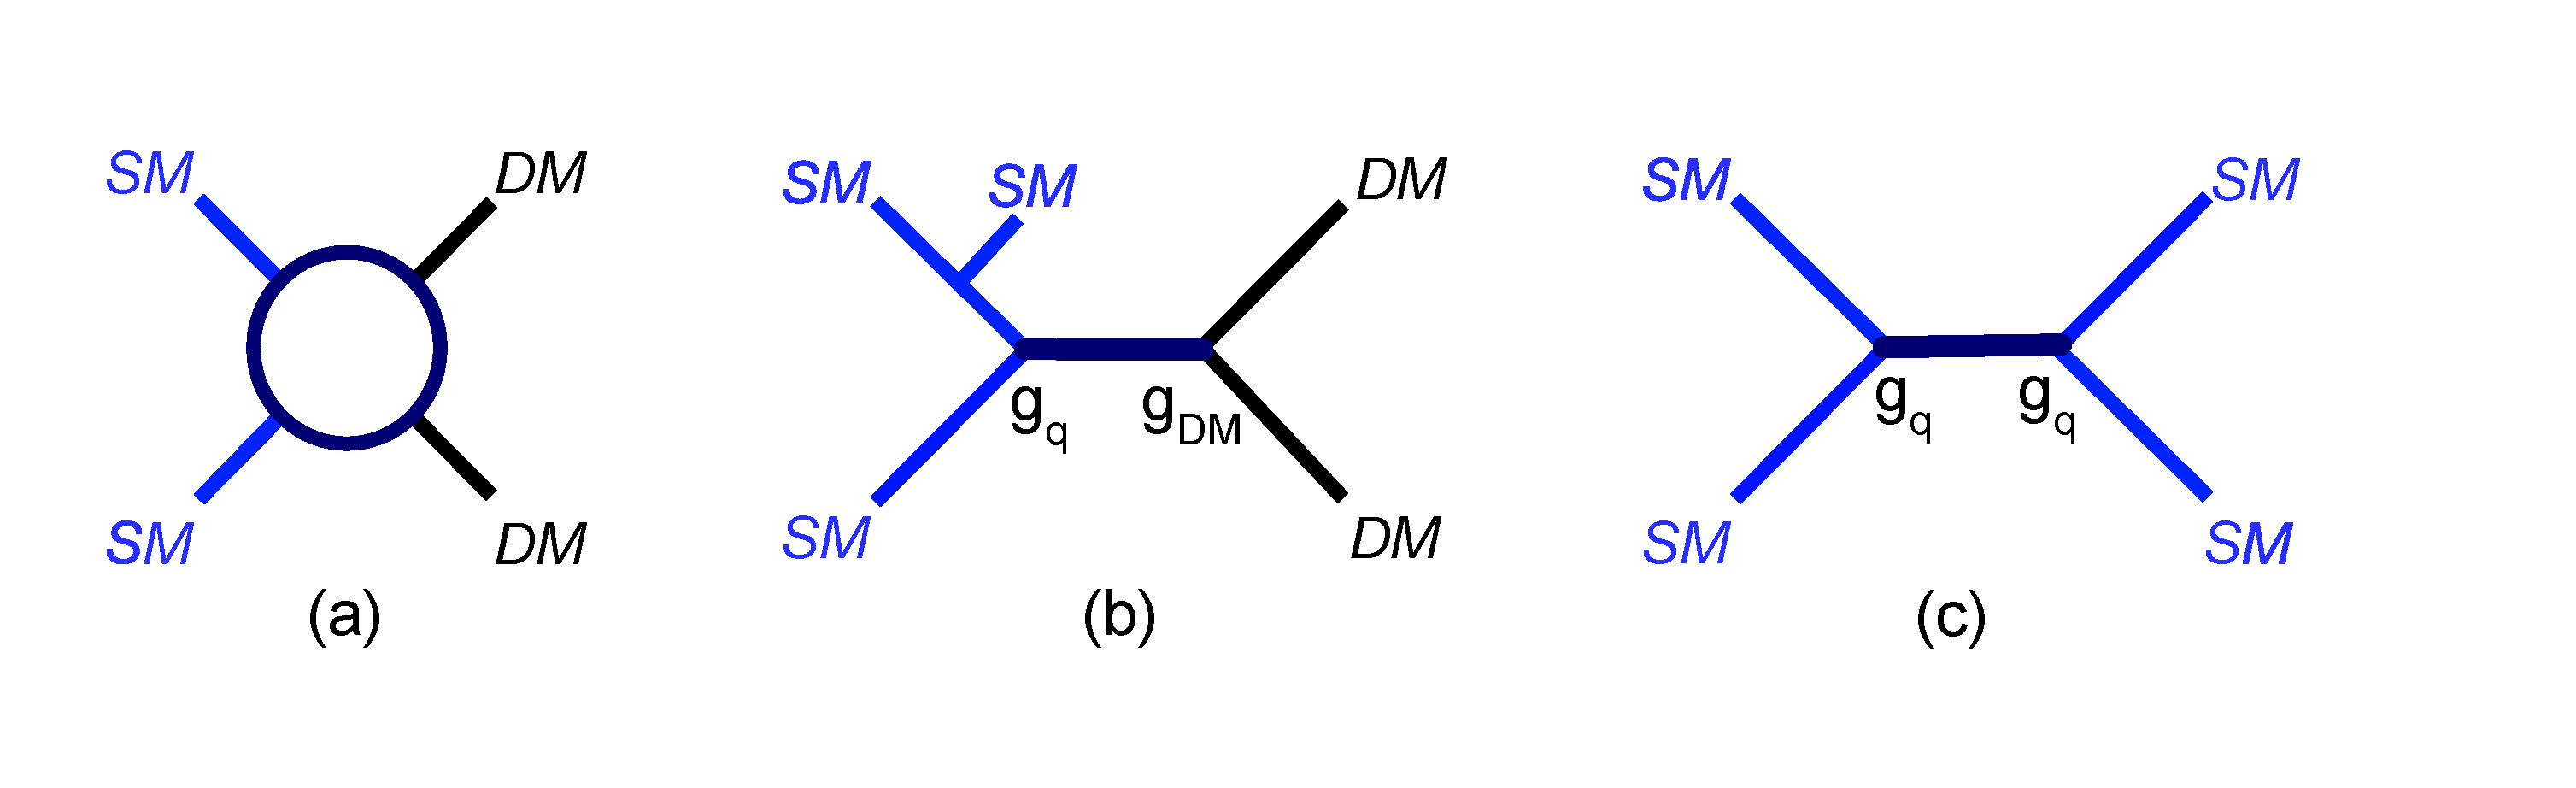
\includegraphics[width=\textwidth]{figures/MonoX.pdf}
\caption{Sketches of (a) the basic Standard Model (SM) - Dark Matter (DM) interaction at colliders in an effective field theory (EFT), (b) its extension as a basic simplified model where a new mediator particle is exchanged in the s-channel (including an additional energetic object radiated from one of the initial state quarks) and (c) the same simplified model where the mediator decays back into SM quarks. The coupling constant characterizing the mediator-quark interaction strenght is denoted as \gq, while the mediator-DM coupling constant is denoted as \gdm. From~\cite{monoXfig}.}
\label{fig:monoX}
\end{figure}

\subsubsection{Effective Field Theories}
\label{sub:EFT}

\textbf{Effective field theories} (EFTs)~\cite{Goodman:2010ku, Shoemaker:2011vi} are the simplest possible models of DM production at the LHC beyond those described in Section~\ref{sec:HZPortalModels}. A four-point interaction is used to describe the DM production at the LHC in a low-energy approximation of a full theory, similarly to what done when describing the weak interaction through a Fermi process before the introduction of the W and Z bosons~\cite{Fermi2008}. EFT operators were first widely employed to describe DM reactions at colliders at the Tevatron~\cite{Bai:2010hh,Beltran:2010ww}. They were found advantageous because of their model-independence, and since each of the operators encapsulates the phenomenological characteristics of most known types of SM-DM interaction. A sketch of an EFT process at the LHC is shown in panel (a) of Fig.~\ref{fig:monoX}. 

The only parameter characterizing an EFT operator, in addition to the type of DM particle and to the type of SM-DM interaction, is the scale of the contact interaction $\Lambda$. In the case of a $s-$channel completion of the EFT, this interaction scale is proportional to the mass of the mediator particle. If the scale of the DM interaction is sufficiently low with respect to the mediator mass, the phenomenology is the same for the EFT as for its $s-$channel completion. 
This may not always be the case at the LHC, given the high center-of-mass energy collisions: a better description of both theory and phenomenology can be reached when explicitly including the new particles in the model considered~\cite{Buchmueller:2013dya,DeSimone:2016fbz,Berlin:2014cfa}. Certain EFT operators also may suffer from gauge invariance issues at the electroweak scale~\cite{Bell:2015sza}. However, if no completion is available, EFTs are still a good benchmark to motivate the exploration distinct kinematic regions and signatures at the LHC. %Maybe mention that obscure model we have in DMF report?

\begin{marginnote}[]
If a completion of the EFT is not available, procedures describing how to truncate the events where the EFT description is not valid are available~\cite{Racco:2015dxa,Busoni:2014sya,Busoni:2013lha,Busoni:2014haa}. A recommendation on how to present EFT results from LHC searches can be found in~\cite{Abercrombie:2015wmb}.
\end{marginnote}

Run-1 LHC searches privileged EFT operators, while Run-2 searches are limited to using EFT models with a SM singlet and a boson pair, coupled to DM through a contact interaction (see e.g.~\cite{Petrov:2013nia,Berlin:2014cfa}). These models provide a direct SM-DM interaction and motivates searches in final states with a vector boson accompanied by \MET. 
%[TODO CD: find completion: maybe Linda's talk at some old DMWG? AB may have more luck with trilobyte searches]

\subsubsection{Simplified models}
\label{sub:simplifiedModels}
 
%CD: this sentence does not really work
Simplified models of BSM mediation are a natural step beyond effective operators and still map well to the different types of interactions. 

Simplified models resolve the issue of whether a model-independent EFT description is valid at the LHC, even though they are not complete models themselves (e.g. not all the models used are gauge invariant~\cite{Kahlhoefer:2015bea}). Simplified models can be used for comparisons with non-collider DM searches within a clearly specified theory framework. Their use as benchmark models for Run-2 searches also highlights the strength of the LHC in searching for the visible decays of the mediator particle alongside its decays in DM particles, as detailed in the next chapter. 

For a comprehensive review of WIMP simplified models of DM at the LHC, we refer to~\cite{Arcadi:2017kky}, while~\cite{Abercrombie:2015wmb} presents a prioritized list of simplified models that have been used in early LHC Run-2 searches. The prioritized, compact set of benchmark simplified models in~\cite{Abercrombie:2015wmb}, as well as their parameters, have been discussed and agreed upon during a joint experimental and theory effort called the Dark Matter Forum (DMF), now Dark Matter Working Group within the LHC Physics Centre at CERN (LPCC)~\cite{DMWG}. 

\begin{marginnote}[]
The DMF was built starting from the discussion of various communities in Refs.~\cite{Yavin:14092893,Malik:2014ggr,Abdallah:2015ter}. All models covered in~\cite{Abercrombie:2015wmb} are available on the DMF git repository. Add reference. 
\end{marginnote}

In the simplified models chosen as benchmarks for the first LHC Run-2 searches, only one extra particle is added to the the DM and SM particle spectra. In general, this particle mediates the DM-SM interactions. If neutral, the mediator particle is singly-produced at the LHC, and decays in pairs of DM particles due to the $Z_2$ symmetry as well as in pairs of SM particles. If the mediator is colored, it can lead to a $t-$channel exchange between an incoming LHC parton and the DM particle. The phenomenology of colored mediators of DM is akin to that of SUSY models with a squark exchange~\cite{Papucci:2014iwa,An:2013xka,Bell:2012rg} with some differences that we will review later in this section. 

Early LHC searches have initially privileged $s-$channel resonances as benchmark models, as a generalization of the simplest portal models described in the previous section. Resonances decaying in two bodies
%, be those visible or invisible particles, 
are a simple, attractive benchmark to be directly produced at particle collider that has just increased its center-of-mass energy. These resonances can be classified according to their spin: spin-1 vector or axial vector mediators (also called Z'), scalar mediators (termed $\phi$ in the following) and spin-2 vector mediators. This review does not cover in detail spin-2 mediators as they have not yet been adopted as benchmark models by LHC searches, even though they produce diboson signatures that are not present in other models. More information on spin-2 mediators can be found in e.g. Refs.~\cite{Kraml:2017atm,Han:2015cty}.

%CD question: introducing parameter scans is too long. 
%CD gut feeling: it would be good to have some pictures to break this up? 
%CD TODO: mention relic for all of these? 
%CD maybe would prefer to move "when do we see this at the LHC" to the next section? 

%%%s-channel
%General
\textbf{Massive spin-1 bosons with axial or axial vector couplings} to SM and DM particles~\cite{Shoemaker:2011vi} are common in many theories, beyond those of DM mediation. They can be considered as heavy copies of the SM Z boson that arise from breaking of larger gauge groups, and as such they can be contained in larger models. A relevant characteristic of this model for LHC phenomenology is that if the Z' couples to quarks (as it needs to, in order to be produced at the LHC), then it must have visible decays back into quarks. This opens a new avenue for searches of this new particle in dijet signatures with sensitivity in early LHC data, complementing searches for excesses of missing transverse momentum. 

%Parameters
The simplest incarnation of kind of model, where the Z' only couples equally to each kind of quarks and to DM, is fully defined given the nature of the Z' couplings (vector, axial vector or mixed), their magnitude (\gq and \gDM), the mass of the DM particle \mdm and the mediator mass \mmed. The nature of the Z' couplings (vector, axial vector or mixed) does not change the LHC phenomenology, but changes the comparison of LHC results to DD and ID searches. Axial vector are the most widely used LHC benchmarks as DD rates are suppressed. [CD: specify more?]. 

%Additions: Higgs and Z' models
Vector and axial vector mediator models can include couplings of the Z' to the Higgs boson, so that the Z' boson can acquire mass through a new baryonic Higgs $h_B$~\cite{Berlin:2014cfa}. This collapses to the simpler vector model in the limit of very heavy Z' mass. When the interaction between the Z' and the SM Higgs is relevant, it can be parameterized using the Z'-SM Higgs coupling \ghZprimeZprime and the mixing angle between the SM Higgs and the baryonic Higgs, \sinthetab. 
%which in turn is a function of the vacuum expectation value of $h_B$. 
This model can also lead to mono-Z signals, if the Z' is allowed to interact with the Z and the photon through kinetic mixing, 
but this interaction has so far been neglected in LHC Run-2 searches. 
%CD: is there a paper by Vichi on this topic? Can't find it
A Z' can also be embedded in a Type-II Two-Higgs Doublet Model (2HDM), where it does not decay directly into DM but instead decays into a new pseudoscalar $A^0$ and a SM Higgs boson with a coupling \gZprime~\cite{Berlin:2014cfa,Liew:2016oon}. Here the model parameter space is more complex, even when the one of the Higgs from the doublets is the SM Higgs (alignment limit). This model includes a mixing between the Z' and the SM Z boson that is proportional to the ratio between the vacuum expectation values of the new Higgs doublets ($tan \beta$). 

%Problems
In certain region of this parameter space, especially at low mediator masses, the leptophobic Z' model can satisfy the relic density constraints~\cite{Chala:2015ama}. However, if taken in isolation, these models are  non-renormalizable, and the axial vector model violates perturbative unitarity in certain regions of the parameter space (see Ref.~\cite{Boveia:2016mrp} and references therein) if \mdm is larger than \mmed. 
%CD: and references therein = maybe we should cite original papers? 

%General, reasons for doing it at the LHC
If the mediator is a real scalar or a pseudoscalar singlet, it can have tree-level interactions with DM.
\textbf{Color-neutral scalar and pseudoscalar bosons} mediating SM-DM interactions (see e.g. Refs.~\cite{Buckley:2014fba}) take advantage of the theoretical and experimental body of knowledge that led to the recent discovery of another scalar boson, the Higgs boson. Minimal Flavor Violation dictates that the coupling of these new bosons to fermions should be proportional to those of the Higgs boson to escape flavor constraints (see Ref. ~\cite{Dolan:2014ska} for a description of remaining constraints for pseudoscalar searches), and therefore that their visible decays should be dominated by heavy-flavor quarks. Other parallels with LHC Higgs phenomenology are the importance of loop-induced couplings to gluons in the production of scalar and pseudoscalar mediators~\cite{Haisch:2015ioa,Mattelaer:2015haa} and the associated production of the mediator together with heavy flavour quarks~\cite{Buckley:2014fba}. Scalar and pseudoscalar models have much lower cross-sections than their vector and axial vector counterparts in the same fashion as the Higgs production cross-section is suppressed with respect to the Z cross-section in the SM, but the associated heavy quarks provide experimental handles that make those models testable at the Run-2 LHC. Single top signatures are also in reach of LHC searches~\cite{Pinna:2017tay}, as they are kinematically favored even though their production cross-section is generally lower with respect to the associated production of a pair of top quarks. %CD: this is interesting and new, but may be cut if we need to cut. 

%Parameters
Color-neutral scalar and pseudoscalar models are fully defined given the masses of the DM particle and of the mediator, the nature of the $\phi$-DM couplings (\gdm) and $\phi$-fermion (\gq) couplings. Following the convention in~\cite{Abercrombie:2015wmb}, \gq is a pre-factor to the Yukawa couplings of the mediator to fermions and it is considered equal for all quarks in early LHC searches. 
The LHC kinematics of models with scalar and pseudoscalar mediators assuming the same couplings is degenerate. Since the pseudoscalar model has been favoured for the interpretation of the DAMA and galactic center excess~\cite{Arina:2014yna,Agrawal:2014una} and collider searches are favored when comparing to DD~\cite{Banerjee:2017wxi}, LHC searches have privileged this choice and considered the associated scalar boson as decoupled at higher energies. 

%Additions: Higgs models
\begin{marginnote}[]
\vskip-100pt
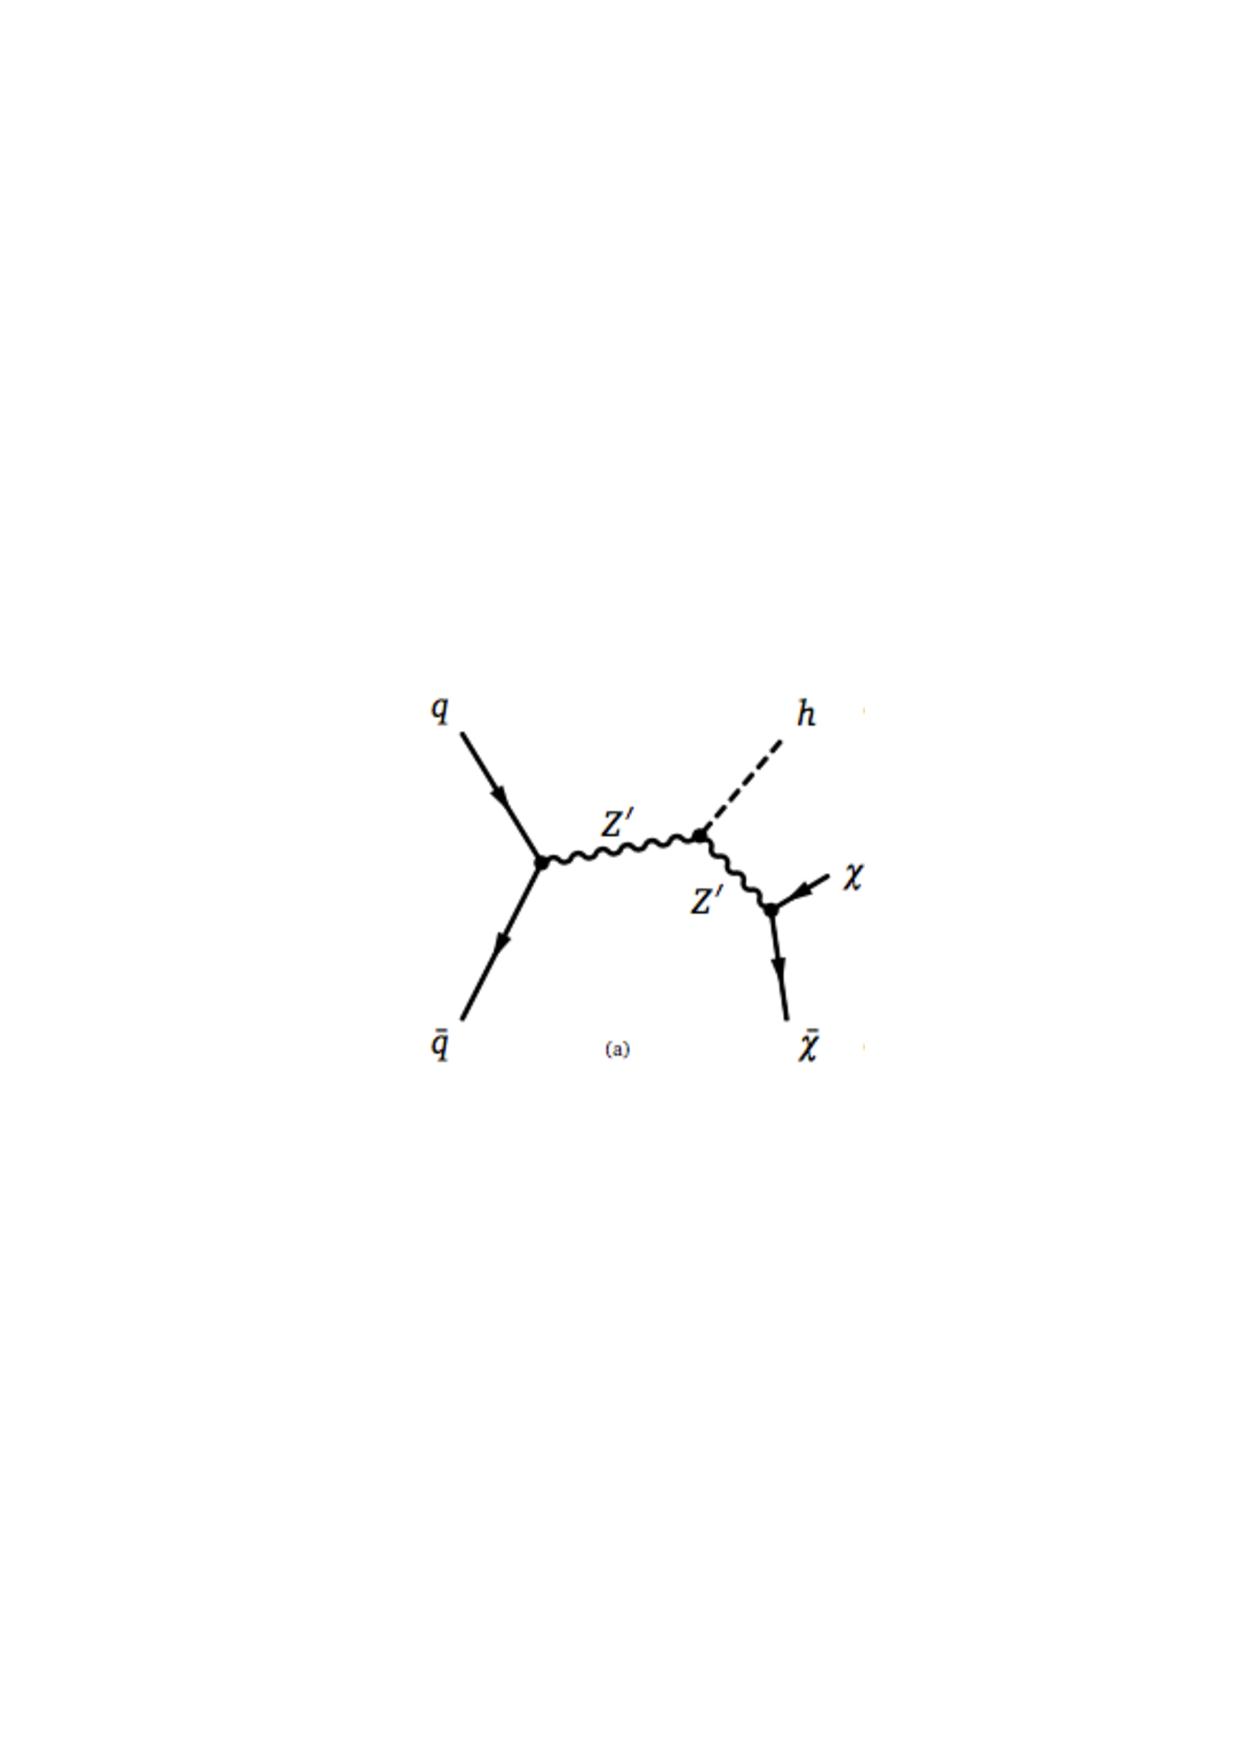
\includegraphics[width=0.5\textwidth]{figures/test-feynman.pdf}
\vskip-100pt
Feynman diagram testing things. We could do this and it's informative, but positioning will be a pain. 
\end{marginnote}

%CD: this needs a feynman diagram otherwise one gets confused
In the most general scalar potential, the scalar can couple to DM through a Higgs portal~\cite{Berlin:2014cfa}. The scalar mediator mixes with the SM Higgs boson with a mixing angle \sinthetahS and with a new physics coupling $b$ that can be set to unity, and to DM through a Yukawa term as above. This model adds mono-Higgs signals to the signatures of the scalar model without Higgs couplings. The mixing angle is constrained from current Higgs precision measurements to be \sinthetahS $<$ 0.4, and the LHC kinematics does not depend on this mixing angle. Couplings to other MS particles, notably EW gauge bosons, can also be added as a consequence of electroweak symmetry breaking as in ~\cite{Bauer:2016gys,Englert:2016joy}. The signatures of this latter model include invisible decays of the Higgs boson if the DM particle is lighter than the SM Higgs, as well as signals of Higgs and vector bosons plus missing transverse momentum at tree level. 

%CD: check back on emails with DiFranzo

%Problems
If the mediators are pure SM singlets, the model is not invariant under $SU(2)_L$~\cite{Bell:2016ekl}. 
%Maybe add Uli/No/etc's papers here?
To restore gauge invariance, the mediator needs to mix with the Higgs sector, introducing further complexity of interactions. However, as we will see in Sec.~\ref{sec:LessSimplifiedModels}, this complexity does not translate into significant changes in the LHC kinematics of the simplest models, but rather adds extra signatures for LHC searches.

%%%t-channel, colored
%General
\textbf{Scalar and pseudoscalar bosons that possess a $Z_2$ charge} take simplified models used at the LHC beyond $s-$channel SM-DM interactions~\cite{Bai:2013iqa, Papucci:2014iwa, An:2013xka, Bell:2012rg} as they mediate the interaction between a DM particle and a SM quark. Models including color triplets of this kind have historically been called $t-channel$ models, but their diagrams are not exclusively of simple $t-$channel mediation. In these particular diagrams, a scalar that is colored under SU(3) is exchanged, analogously to a squark exchange in the MSSM where only squarks and neutralino are light.
With respect to the $s-$channel mediator models, models with a colored scalar mediator have a broader set of multi-jet signatures and kinematic features that make it interesting in terms of LHC phenomenology~\cite{Abercrombie:2015wmb}. %This will be substituted by the DMWG write-up if it comes in time. 
Another handle for LHC searches is the radiation of a Z boson by the right- and left-handed mediators, as well as a W boson by the left-handed mediator~\cite{Bell:2012rg}. 

%Parameters
The definition of the parameter space for colored mediator models requires setting the mass of the mediators and of the DM particle. The mediator mass is set equal for all mediators due to the MFV assumption, and the mediator must be heavier than the DM particle to ensure DM stability. 
%Requirement of the width: mChi^2+mq^2<=Mmed^2
The coupling between DM and quarks \gdmq in LHC searches have been set to be universal but only to the first two quark generations, violating MFV. 
%CD: the following sentence does not have a source, and the Bell model only uses left-handed quarks. This is a question for Millie and the theorists present tomorrow. 
However, if only right-handed, down-type quarks are considered, flavour constraints still do not exclude a significant part of the parameter space~\cite{Abercrombie:2015wmb}. 

As opposed to the MSSM, the coupling between DM and quarks in this simplified model is not a priori fixed or constrained by the necessity of fitting within a more complex, self-consistent particle spectrum. The couplings required for this model to satisfy the relic density are generally higher than what used by SUSY models. 
%Citation to MG's studies?
Couplings to vector bosons also allow the mediator to radiate a W or a Z, leading to LHC signatures that can be targeted by specific searches~\cite{Bell:2012rg}. 
%Problems 
More sophisticated models that satisfy the full SM gauge symmetry and MFV include third generation couplings and lead to two independent mediators and couplings are described in Ref.~\cite{Ko:2016zxg}. 
The parameters and couplings of this model have also been tuned to describe the gamma ray excess and motivate searches with a single $b-$quark in the final state~\cite{Agrawal:2014una}, leading to a similar phenomenology as the MSSM with a light bottom squark and neutralino. 
%Top-flavored models also exist in literature but have not been used as benchmarks in LHC searches. 

\subsubsection{Consequences of $s-$channel mediated models: visible decays}
\label{sec:MediatorSearches}

As mentioned in the earlier section, if the mediator particle is produced from from interactions of
quarks and gluons, it will also decay in quarks and gluons. 
For this reason, it is worthwhile that collider experiments not only search for
the invisible Dark Matter particles, but also probe directly the interaction between Standard Model and 
Dark Matter particles by searching for the visible decays of the particles that mediate it, as shown 
in Figure~\ref{fig:monoX} (c) and summarized in e.g. Refs.~\cite{Liew:2016oon,Fairbairn:2016iuf}. 

%CD cite the following
%Coupling--mass mapping of di-jet peak searches, 10.1103/PhysRevD.88.035021 ok
%Searches for Dijet Resonances at Hadron Colliders, 10.1142/S0217751X11054905 in the experimental part, i would say
%Searching for Low Mass Dark Portal at the LHC, 10.1016/j.dark.2013.03.002 ok
%Constraining Dark Sectors with Monojets and Dijets, 10.1007/JHEP07(2015)089 ok
%Constraints on Z? models from LHC dijet searches and implications for dark matter - https://arxiv.org/pdf/1605.07940.pdf -> ok

Dijet searches are sensitive to vector and axial vector DM mediators decaying 
exclusively to jets with couplings that would satisfy relic density constraints~\cite{Chala:2015ama},
but also to new, unknown particles that might be created when crossing 
the threshold of a new energy scale. For the same reason, 
it is not possible to claim a discovery of DM mediators at the LHC without
corresponding excesses in invisible channels and non-collider experiments. 
Nevertheless, these benchmark models have motivated novel search techniques
to look for low-coupling, low-mass resonances below the TeV scale that would
have otherwise not been explored in early Run-2 data due to experimental difficulties~\cite{An:2012ue,Dobrescu:2013coa}. 

The leptophobic vector and axial vector simplified models described in \ref{sub:simplifiedModels} 
are however not always theoretically viable, as lepton decays are needed for gauge invariance
or are included through radiative corrections leading to a mixing between the Z' and the Z 
(see Ref.~\cite{Albert:2017onk} and references therein). A simple extension of the leptophobic vector
and axial vector models allows the mediator to decay into leptons at tree level. 
As explained in the next sections, dilepton resonances are often more sensitive than dijet resonances
at the LHC. Decays of the spin-1 mediator into neutrinos are also required by gauge invariance, and add 
an invisible decay channel that can enhance signatures of missing transverse momentum, depending on
the size of the couplings~\cite{Albert:2017onk}. 

%All citations from DMF, probably want to save citations for later
%They are sometimes necessary in order to construct a consistent theory, for example in minimal completions of the axial-vector model [11, 12] or in models with extended Higgs sectors [13, 14]. They often appear in anomaly-free spin-1 mediator models [15], see also Section 3.3.2 of [7]. They may also be induced through radiative corrections (e.g. through quark loops that lead to Z??Z mixing). The near-ubiquity of lepton couplings in full theories motivates including them when searching for visibly-decaying spin-1 mediators.

%Generic resonance searches sensitive to a broad range of theoretical models 
%are already the focus of LHC. 

\subsubsection{Less simplified models}
\label{sec:LessSimplifiedModels}

The initial list of models recommended to the experimental collaboration by the Dark Matter Forum described above is a first set of simple, mostly tree-level processes targeting early Run-2 searches. Targeting one simplified model at a time however does not cover the full complexity of LHC signatures and kinematic distributions in more complete models. Exclusively considering simplified models therefore presents the risk of missing important search targets. Moreover, UV-complete models are important and interesting as they offer solutions to SM problems beyond DM, as in the case of SUSY that will be discussed in the following section. 

There are a large number of these "less-simplified" models in literature, and very few of them have been explored directly by LHC searches considering them as benchmarks. In this review we will only sketch the main characteristic of a small selection of models within our grounding assumptions. This selection has different kinematic consequences and different signatures with respect to the simplified models used by Run-2 LHC searches so far. 

\textbf{Co-annihilation} models add one extra particle to the dark sector, generally close in mass to the DM particle. Examples can be found in Refs.~\cite{Buschmann:2016hkc,Baker:2015qna,Khoze:2017ixx}. The strong interaction between these two DM states drives the cosmological history~\cite{PlehnLecturesDM}, as processes involving both DM particles can efficiently annihilate DM into SM particles. In terms of LHC phenomenology, coannihilation models produce signatures of missing transverse energy and multiple hadronic jets accompanied by multiple resonant or non-resonant hadronic jets, in some cases untested by current searches~\cite{Buschmann:2016hkc}. In other cases, the small mass splitting between the two particles forces the decay of the next-to-lightest particle into the lightest particle to be kinematically suppressed, in turn leading to a sizable lifetime for the next-to-lightest particle~\cite{Khoze:2017ixx}. The late decays of the coannihilation partner give an additional experimental handle that can be used for LHC searches, as described in the next chapter.  
%Dark terminator needs Majorana particle, not mentioned although the idea of vector + scalar is interesting beyond LianTao's 2HDM
%Other~\textbf{models with two mediators, a scalar and a vector} with small couplings to SM particles have been developed to escape existing LHC constraints~\cite{Duerr:2016tmh}. 

%OOutline said monotop, but I don't know where to fit those because they don't necessarily have much to do with anything we talked so far? i would be happier to talk about monotop searches in terms of Priscilla/Deborah's studies. 

%OOutline said gluphilic, but we cited it above and we need to save space

The \textbf{evolution of scalar models} has also attracted the attention of both theory and experimental LHC community. The simplified scalar and pseudoscalar models described in Sec.~\ref{sub:simplifiedModels} are not self-consistent, if considered as stand-alone models they only focus on one experimental signature at a time. They are not considered the best benchmark model to make the most of %CD: bleurgh
the search opportunity offered by a machine that is sensitive to scalar particles with couplings of the order of those of the Higgs boson.
The first step towards more consistent scalar and pseudoscalar models is the addition of Higgs couplings and coupling to vector bosons that naturally stem from gauge invariance, as described above and in~\cite{Bauer:2016gys,Berlin:2014cfa}. A further refinement is to embed the scalar/pseudoscalar model in a more complete theory, namely a Two-Higgs Doublet Model (2HDM)~\cite{Bauer:2017ota,Ipek:2014gua,No:2015xqa,Goncalves:2016iyg,Bell:2016ekl}. 
%%Overkill?
%[1] M. Bauer, U. Haisch, F. Kahlhoefer, CERN-TH-2017-011, DESY-17-010 [arxiv:1701.07427 [hep-ph]].
%[2] S. Ipek, D. McKeen and A. E. Nelson, Phys. Rev. D 90, no. 5, 055021 (2014) [arXiv:1404.3716 [hep-ph]].
%[3] J. M. No, Phys. Rev. D 93, no. 3, 031701 (2016) [arXiv:1509.01110 [hep-ph]].
%[4] D. Goncalves, P. A. N. Machado and J. M. No, arXiv:1611.04593 [hep-ph].
%[5] N. F. Bell, G. Busoni and I. W. Sanderson, arXiv:1612.03475 [hep-ph].
In these models, the new scalar or pseudoscalar mediator mixes with the Higgs partners rather than with the SM Higgs, so that the model is still compatible with Higgs measurements. 2HDM+scalar/pseudoscalar have an interesting phenomenology that is not dominated by jet+missing transverse momentum searches but rather by the results of searches of Higgs or EW bosons+MET. A richer span of experimental signatures permits to expose uncovered regions in the parameter space of the model, as well as to highlight the complementarity between final states. 2HDM models developed for LHC searches focus on a Yukawa structure of Type-II, where the couplings are the same as the MSSM. The particle content of this model includes two CP-even bosons (one of which is the SM Higgs boson), two CP-odd bosons (of which one is the pseudoscalar DM mediator, privileged because it escapes DD constraints), two charged Higgs boson and the DM particle. Masses and couplings of these models are chosen to respect vacuum stability~\cite{No:2015xqa}, electroweak and flavour constraints, as well as to highlight the complementarity of the various experimental signatures. Depending on the parameter chosen, this model can satisfy the relic DM density, in general with values of \mdm above 100 GeV.   

%Sam's LianTao's 2HDM checks
%https://docs.google.com/presentation/d/10R9XJaoMDEhXKhd_Wx9yMXEaPl4uXR8IcmuTeLancvg/edit#slide=id.g217998804d_0_47

\subsection{Supersymmetric models and other theories}
\label{sec:SUSYModels}

[left for AB, see ooutline]

R-parity conservation makes the neutralino a viable DM particle candidate. 

Other BSM theories including DM particle candidates that are not covered in this review are extra dimensions~\cite{Hooper:2007qk}, and DM as sterile neutrino~\cite{Adhikari:2016bei}. For AB who has book: See Bertone's book for non-SUSY candidates at the EW scale. 

\subsection{Long-lived particle models}
\label{sec:LLPModels}

%CD: this is very clumsy but in the spirit of blurting everything out, here it is

As discussed in the introduction to this chapter, the LHC does not directly detect DM, but rather uses visible objects to signal the presence of non-interacting, long-lived particles that escape detection. If the particle does not decay, then it is a good DM candidate. In many non-WIMP, dark sector models, one can postulate the existence of DM particles as well as other particles with lifetimes not long enough to be cosmologically stable. Those particles would escape conventional detection by collider experiments, as they e.g. decay half-way through the detector, and still lead to signatures of missing transverse momentum. 
However, these dark sector particles usually do not carry sufficient energy to be observed in this way, so experiments must devise methods that specifically target those non-standard decays. These will be discussed in Chapter~\cite{sec:05_Future}.

%This is probably too much?
%taken some examples from: https://indico.cern.ch/event/606421/contributions/2558018/attachments/1445296/2226369/long_lived_overview.pdf
The main mechanisms for a partner particle to acquire a long lifetime are related to the suppression of its tree-level decays when:
\begin{itemize}
\item the partner particle has a large mass compared to its parents and decay products, so the decay proceeds off-shell, as in the case of e.g. the W-mediated pion decay in the SM;
\item the partner particle can decay to the DM particle but won't do so frequently due to the small mass splitting, as in the case of coannihilation;
\item when the couplings between the partner particle and either SM or DM particles are small, as in the case  of the Cabibbo-suppressed B-meson decays in the SM. 
\end{itemize}

In this review, we only sketch two examples of the third case, as it connects directly with the simplified models described in Sec.~\ref{sub:simplifiedModels}. If the only connection between the DM and SM is the new mediator particle, and DM can annihilate directly to BSM mediators and not viceversa (as \mdm $>$ \mmed), then the couplings of the mediator to the SM can be arbitrarily small. This happen for example when introducing a U(1)' symmetry mediated by a vector boson (a "dark boson"), leading to coupling $\epsilon$ through kinetic mixing, or when adding a scalar boson (a "dark Higgs") that only couples to the SM via a Higgs portal or via mixing with a heavy pseudoscalar in 2HDMs with a coupling $k$. 
%The latter model is interesting because ID is suppressed, but it's called the nightmare scenario.
In both these cases, the mediator (a "dark boson") can be long-lived~\cite{Pospelov:2007mp}, and its visible decays into SM particles or associated production with a SM boson provide the main collider handle~\cite{Curtin:2014cca}. 
%Z width, contact interactions
There is a large possible dark boson mass range that is still compatible with thermal freeze-out, from 1.5 GeV to 40 TeV~\cite{Das:2010ts}, and it can be probed by complementary experiments including present and future colliders. Another mechanism for generating the relic density that is compatible with very weak SM  interactions such as those of dark photons is the freeze-in scenario (see e.g.~\cite{Co:2015pka,Bernal:2017kxu}), where DM is produced from the thermal bath but never reaches equilibrium. CD: I don't understand this yet. 

Another bottom-up approach adopted in~\cite{Buchmueller:2017uqu} is to impose masses and couplings for the models described in~\ref{sub:simplifiedModels} so that they include a long-lived particle. The categorization of the models by production operator and final state permits a more systematic set of benchmarks for this kind of signatures. These models can then be mapped onto more complete theories. No attempts have yet been made however to connect these models to cosmological history. 
